%\chapter[Algorithme de propagation d'interfaces régulières \piecewise]{Algorithme général pour la propagation d'interfaces régulières \piecewise}
\chapter[Algorithme général pour la propagation d'interfaces $\contgeom{1}$ \piecewise]{Mise au point d'un algorithme général pour la propagation d'interfaces régulières \piecewise}
\label{chap:algo_general}

%Objectif : proposer un algorithme de construction de l'EdB sous la forme d'un nouveau modèle \brep\ à partir du modèle \brep\ de l'interface courante. 
%Pour cela, on tire d'abord des observations sur lesquelles on se basera pour construire dans un premier temps une pseudo-EdS, que l'on traitera dans un second temps afin d'obtenir l'EdB. 
%Dans ce chapitre, on explicitera une partie des algorithmes utilisés mais les détails de la mise en \oe uvre numérique feront l'objet du chapitre suivant.

Dans ce deuxième chapitre on propose un algorithme basé sur le principe de Huygens avec condition d'entropie pour simuler la propagation d'une interface décrite dans le formalisme de la représentation par les frontières. 
L'objectif est donc de construire un nouveau modèle \brep\ décrivant l'enveloppe des boules centrées sur l'interface à un instant donné.
Pour cela, on tire des observations sur lesquelles on se basera pour construire dans un premier temps un sur-ensemble de l'EdB duquel on retirera dans un second temps les régions qui ne figure pas sur l'EdB.
\par
Dans ce chapitre, on explicitera chaque étape de l'algorithme mais les détails de la mise en \oe uvre numérique feront l'objet du chapitre suivant.


\setlength{\imagewidth}{74mm}
\setlength{\imageheight}{\imagewidth}
\def\trmask{0.82}
\begin{figure}
  \centering
  \tikzset{x=\imagewidth, y=\imageheight,
  	img/.style={anchor=south west, inner sep=0}}
  %
  \hspace*{\fill}
  \subbottom[Modèle \brep\ de l'interface.]{
	\begin{tikzpicture}
		\figEoBBrep{1}{0}{0}
%		\draw[blue, dashed] 
%			(current bounding box.south west) --
%			(current bounding box.south east) --
%			(current bounding box.north east) --
%			(current bounding box.north west) -- cycle;
	\end{tikzpicture}
  }
  \hfill%
  \subbottom[Modèle \brep\ de l'enveloppe des boules centrées sur l'interface.]{
	\begin{tikzpicture}
		\figEoBBrep{2}{0}{0}
%		\draw[blue, dashed] 
%			(current bounding box.south west) --
%			(current bounding box.south east) --
%			(current bounding box.north east) --
%			(current bounding box.north west) -- cycle;
	\end{tikzpicture}
  }
  \hspace*{\fill}
  \caption{Entrée et sortie de l'algorithme présenté dans le chapitre (REFAIRE).}
  %
\end{figure}

%[Convexité des courbes singulières (foreshadowing Hohmeyer), EdB $\subset$ EdS ($\to$ \autoref{section:principe_huygens}?), notion d'EdS partielle suffisante (ou \guillemets{pseudo-EdS}, \cf notes Huygens)]

\section{Convexité des courbes singulières}
\label{section:def_convexite_courbe_singuliere}
[Objectif : formaliser la notion de convexité d'une courbe singulière de $\Sigma$ (qui servira pour simplifier la construction de l'EdB) et démontrer que la convexité est "continue", \ie que deux segments d'une même courbe singulière, l'un convexe et l'autre concave, sont nécessairement séparés par un point régulier de $\Sigma$]
%\par\bigskip
%\begin{enumerate}
%	\item $\Sigma$ 2-variété donc tout $\p \in \Sigma$ possède un voisinage $\neigborhood$ homéomorphe à un disque
%	\item si $\p$ est à l'intérieur d'une courbe singulière $\Gamma$ de $\Sigma$, alors $\neigborhood = 
%        \left(\neigborhood \cap \Sigma_1\right) \cup
%        \left(\neigborhood \cap \Gamma\right) \cup 
%        \left(\neigborhood \cap \Sigma_2\right)$
%	\item 
%\end{enumerate}
%\def\p{\vit{p}}
%Puisque $\Sigma$ est une variété de dimension 2 sans bord, chaque point $\p$ de $\Sigma$ possède un voisinage $\neigborhood$ homéomorphe à un disque.
%Si $\p$ est situé à l'intérieur d'une courbe singulière $\Gamma$ de $\Sigma$, alors ce voisinage peut être décomposé comme
%\begin{equation}
%    \neigborhood = 
%        \left(\neigborhood \cap \Sigma_1\right) \cup
%        \left(\neigborhood \cap \Gamma\right) \cup 
%        \left(\neigborhood \cap \Sigma_2\right),
%\end{equation}
%où $\Sigma_1$ et $\Sigma_2$ désignent deux nappes régulières (qui peuvent éventuellement être confondues) adhérentes à $\p$ (une à gauche et une à droite de $\Gamma$).
%
%\begin{figure}
%    \centering
%    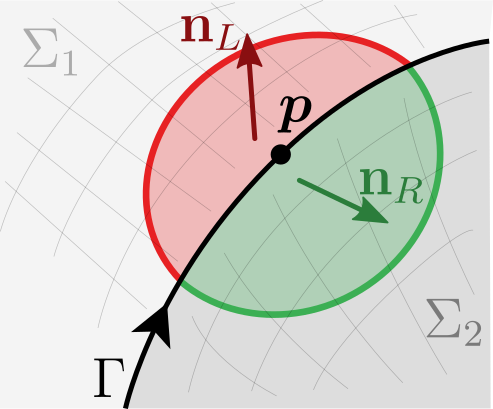
\includegraphics[width=5cm]{voisinage_courbe_singuliere.png}
%    \caption{Voisinage d'un point sur une courbe singulière.}
%\end{figure}



\section{Observations}%/Motivations}
[Objectif : justifier en quoi la construction intermédiaire d'une \guillemets{EdS partielle} (sous-ensemble de l'EdS qui contient l'EdB) permet de simplifier la construction d'un modèle \brep\ de l'EdB en évitant de construire des éléments de l'EdS qui sont trivialement exclues de l'EdB]
\par
définitions : 
\begin{itemize}
	\item \textit{zone d'influence}\footnote{\label{note_vocabulaire_notation}vocabulaire et notation à préciser \ldots} de $H \subseteq \Sigma$ sur l'EdB  (lieu des points de tangence entre $\EoB{\Sigma}{\rho}$ et $\sphere[H][\rho]$)
	\[ \influEoB{H}{\rho} := \EoB{\Sigma}{\rho} \cap \sphere[H][\rho] \]
	\item \textit{EdS propre}\footref{note_vocabulaire_notation} de $H \subseteq \Sigma$ 
	\[ \EdSpropre{H}{\rho} := \closure{ {\EdS{H}{\rho} \setminus \EdS{\boundary{H}}{\rho}} } \]
\end{itemize}
arguments :
\begin{enumerate}
	\item on sait décrire l'EdB simplement de manière \textit{implicite} (\cf \autoref{section:principe_huygens}) mais on cherche à en construire une représentation \textit{explicite}
	\item en revanche, on peut décrire explicitement l'EdS de chaque carreau ($\to$ introduire système définissant l'EdS à 2 paramètres)
	\item il est plus commode de voir l'EdS d'un carreau comme (un sous-ensemble de) la réunion de 10 nouveaux carreaux (intérieur $\to 2$ , bords $\to 4$ et ``coins'' $\to 4$)
	\item si on procède ainsi pour chaque carreau qui décrit l'interface, on construit beaucoup de nouveaux carreaux qui sont redondants, voire même trivialement exclus de l'EdB
	\item la zone d'influence sur l'EdB d'une courbe singulière concave est vide (preuve?) (\ie cette courbe ne contribue pas à l'EdB et peut donc être ignorée)
	\item la zone d'influence sur l'EdB d'une courbe singulière convexe $\Gamma$ est incluse dans la portion de son EdS qui est tangente aux EdS des deux nappes adhérentes à $\Gamma$ (preuve?), on appelle cette portion \textit{pseudo-EdS} de $\Gamma$ et on la note $\pseudoEdS{\Gamma}{\rho}$
	\item si toutes les courbes singulières adhérentes à un point singulier sont concaves alors la zone d'influence sur l'EdB de ce point est vide (preuve?) (\ie ce point ne contribue pas à l'EdB et peut donc être ignoré)
	\item si toutes les courbes singulières adhérentes à un point singulier $\p$ \textit{ne sont pas} concaves (ou bien que $\p$ n'est adhérent à aucune courbe singulière, \eg le sommet d'un cône) on dit que $\p$ est convexe et sa zone d'influence sur l'EdB est la portion de $\sphere[\p][\rho(\p)]$ qui est tangente aux EdS de toutes les courbes singulières adhérentes à $\p$ (preuve?), on appelle cette portion \textit{pseudo-EdS} de $\p$ et on la note $\pseudoEdS{\p}{\rho}$
	\item l'EdB est incluse dans la réunion
	\begin{itemize}
		\item des EdS propres des nappes régulières (qui sont elles-mêmes contenues dans la réunion des EdS propres des faces \brep)
		\item des pseudo-EdS des courbes singulières convexes
		\item des pseudo-EdS des points singuliers convexes
	\end{itemize}
	\item[$\Rightarrow$] on construit d'abord une telle réunion (que l'on appelle \textit{EdS partielle}) puis on en élimine les régions qui sont exclues de l'EdB (au passage on constitue les relations topologiques qui assurent la validité du modèle \brep)
\end{enumerate}












\section{Construction d'une EdS partielle}
\label{section:def_canal_surface}

[Objectif : donner les étapes de la construction d'une EdS partielle sous la forme d'un ensemble de carreaux restreints (paramétrisation + courbes de restriction du domaine paramétrique) avec des relations d'adjacences partielles)]




\subsection{Paramétrisation de l'EdS propre d'une face \brep}% carreau paramétrique restreint}
\label{section:parametrisation_eds_propre_face}
\begin{enumerate}
	\item paramétrisation de l'EdS propre d'un carreau non-restreint
	\begin{enumerate}
		\item rappeler système définissant une EdS propre à 2 paramètres
		\item interprétation : intersection de cercles caractéristiques $\to$ 2 points (\ie 2 nouveaux carreaux), on garde celui dans le sens de $+\unv$ (l'autre est trivialement exclu de l'EdB)
		\item paramétrisation à la Gelston \cite{gelston1995}
		\item différence avec le simple transport suivant la normale (ordre 2 en temps)
	\end{enumerate}
	\item conservation du domaine paramétrique (pas de re-paramétrisation) $\Rightarrow$ coordonnées $(x,y,z)$ des courbes de restriction données directement par la nouvelle paramétrisation
\end{enumerate}

\begin{figure}
	\centering
	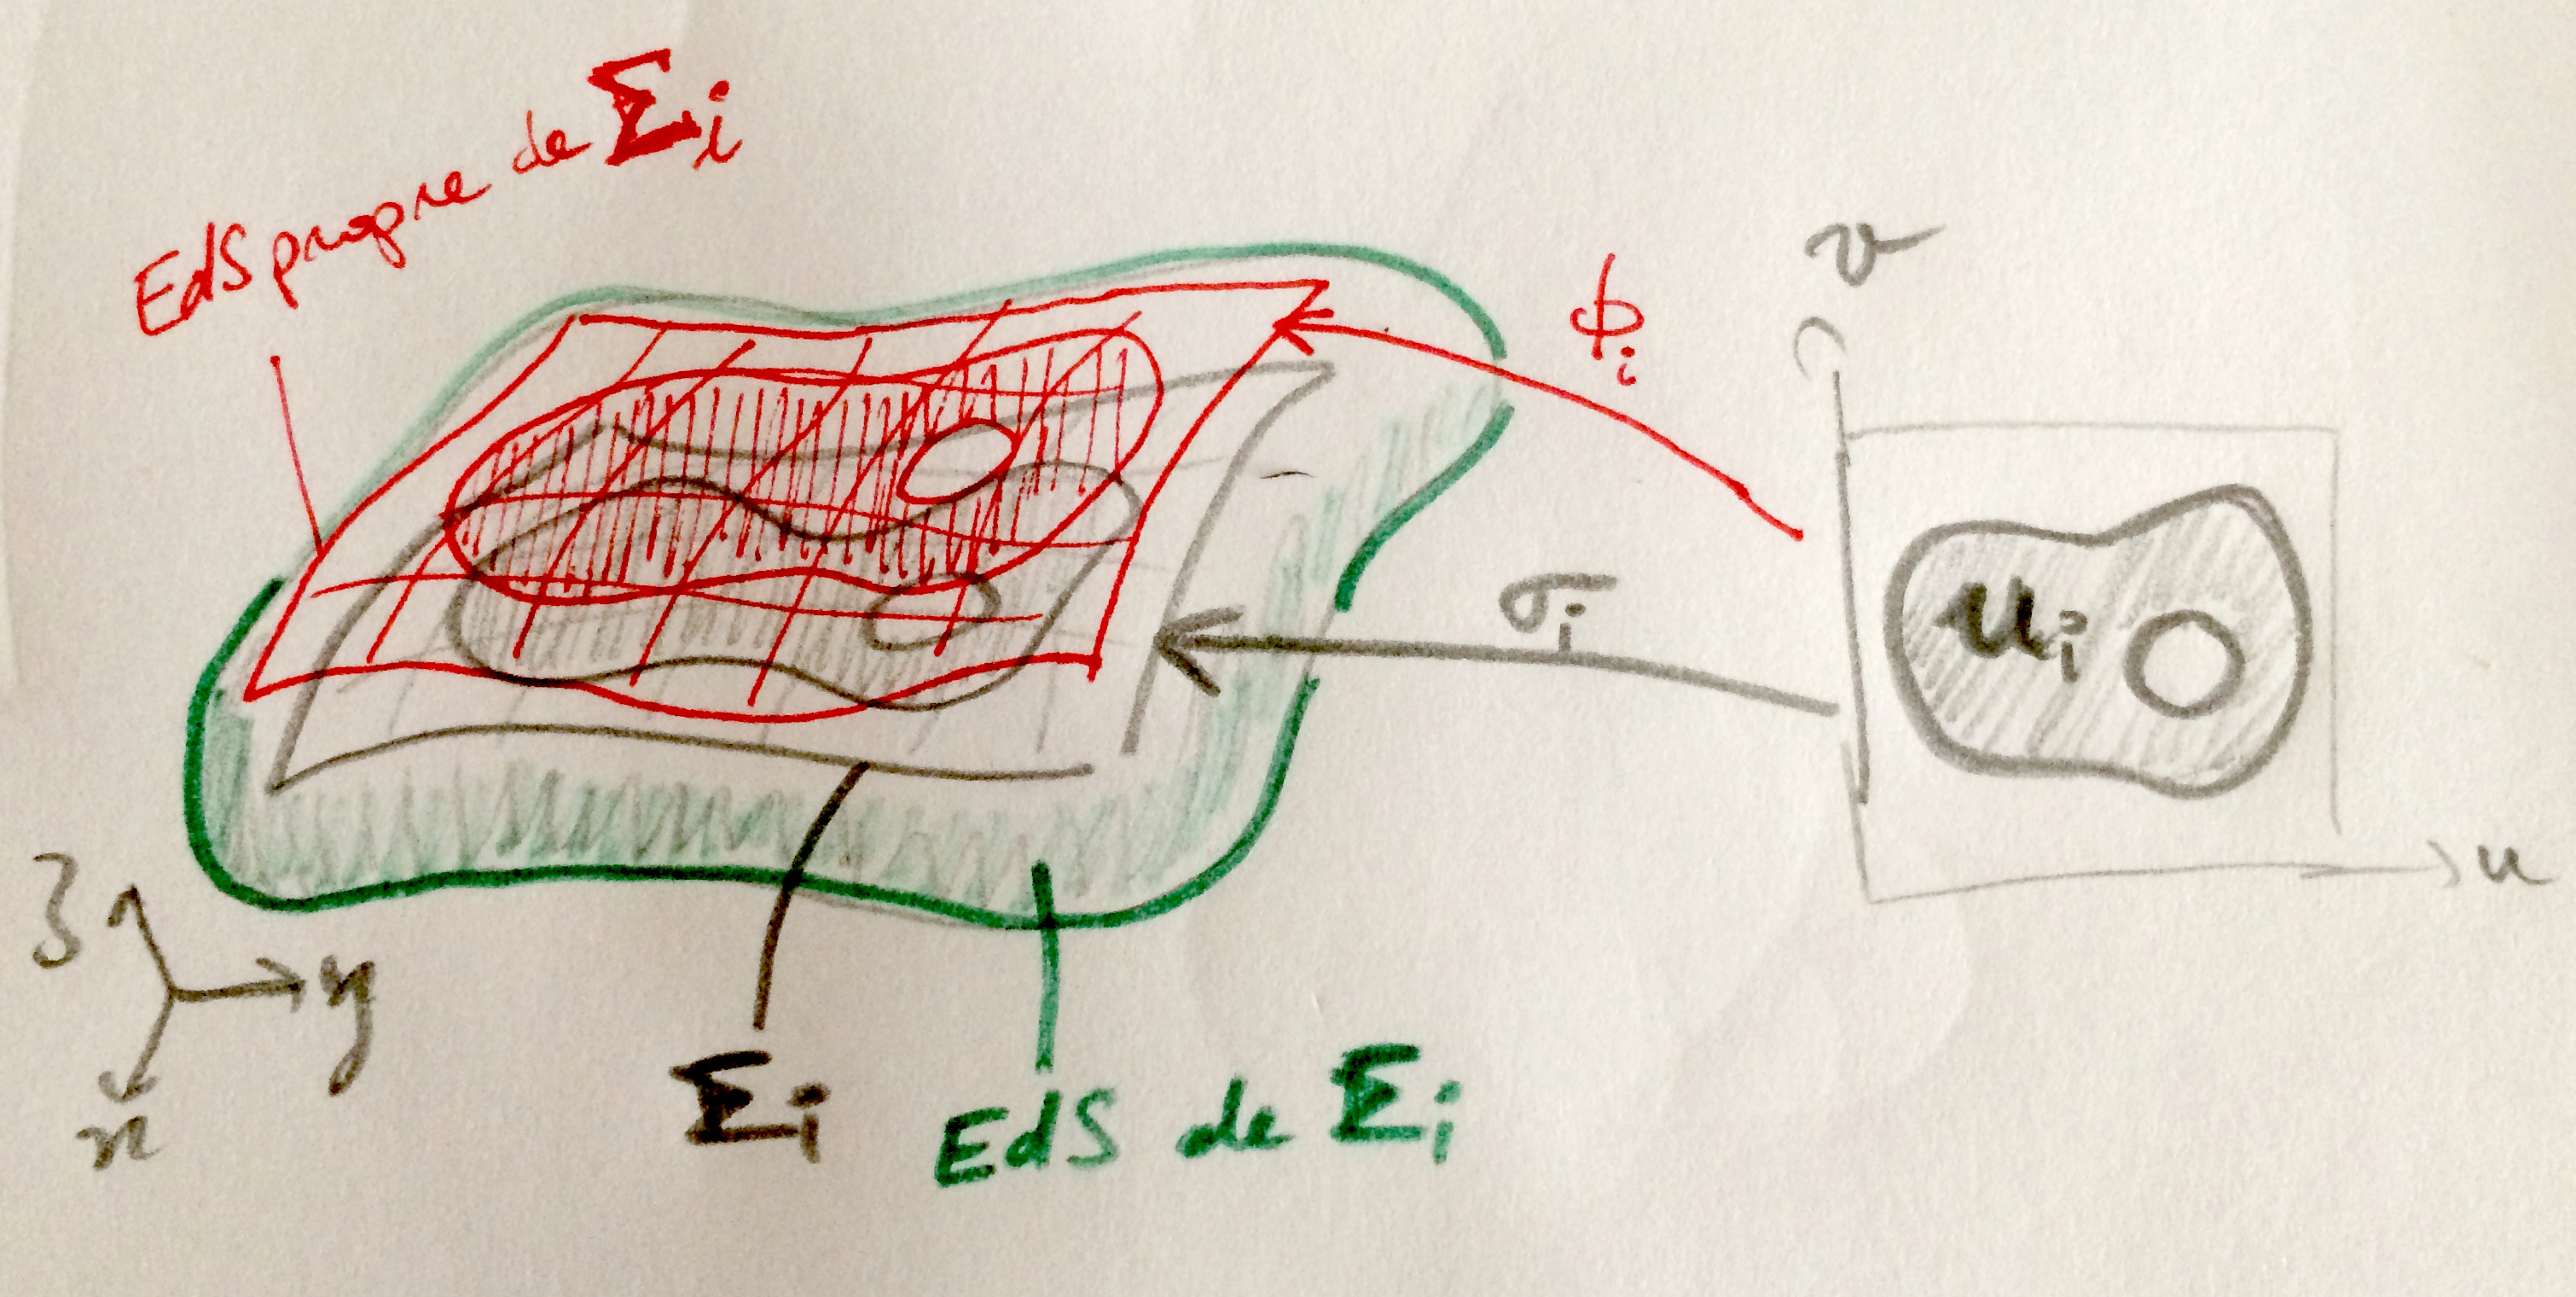
\includegraphics[width=10cm]{EdS_propre_carreau_restreint.JPG}
	\caption{EdS propre d'un carreau paramétrique restreint.}
	\label{fig:EdS_propre_carreau_restreint}
\end{figure}



\subsection{Paramétrisation de la pseudo-EdS d'une arête \brep\ convexe}% arc paramétrique}
\label{section:parametrisation_pseudo_EdS_arete}
\begin{enumerate}
	\item détermination de la convexité de l'arête (signe de $\dotprod{\left(\crossprod{\unv_L}{\unv_R}\right)}{\vrm{t}}$, \cf \autoref{section:def_convexite_courbe_singuliere})
	\item rappeler système définissant une EdS (propre) à 1 paramètre
	\item notion de cercle caractéristique
	\item paramétrisation $\vit{\phi}(u,v) = \vit{o}(u) + r(u)\vrm{r}(u,v)$
	\item restriction à la portion entre les EdS propres des faces incidentes, paramétrisée sur le domaine $\uvdomain = \wdomain \times  \left[ \lo{v}, \hi{v} \right]$
\end{enumerate}

\subsubsection{Paramétrisation de l'EdS propre d'un arc paramétrique}


\begin{figure}
	\centering
	\setlength{\imagewidth}{120mm}%
	\setlength{\imageheight}{0.6857\imagewidth}%
	\definecolor{coloreos}{HTML}{64CF36}
	\definecolor{colorshpere}{HTML}{CD6E33}
	\begin{tikzpicture}[x=\imagewidth, y=\imageheight]
		\node[inner sep=0, anchor=south west] {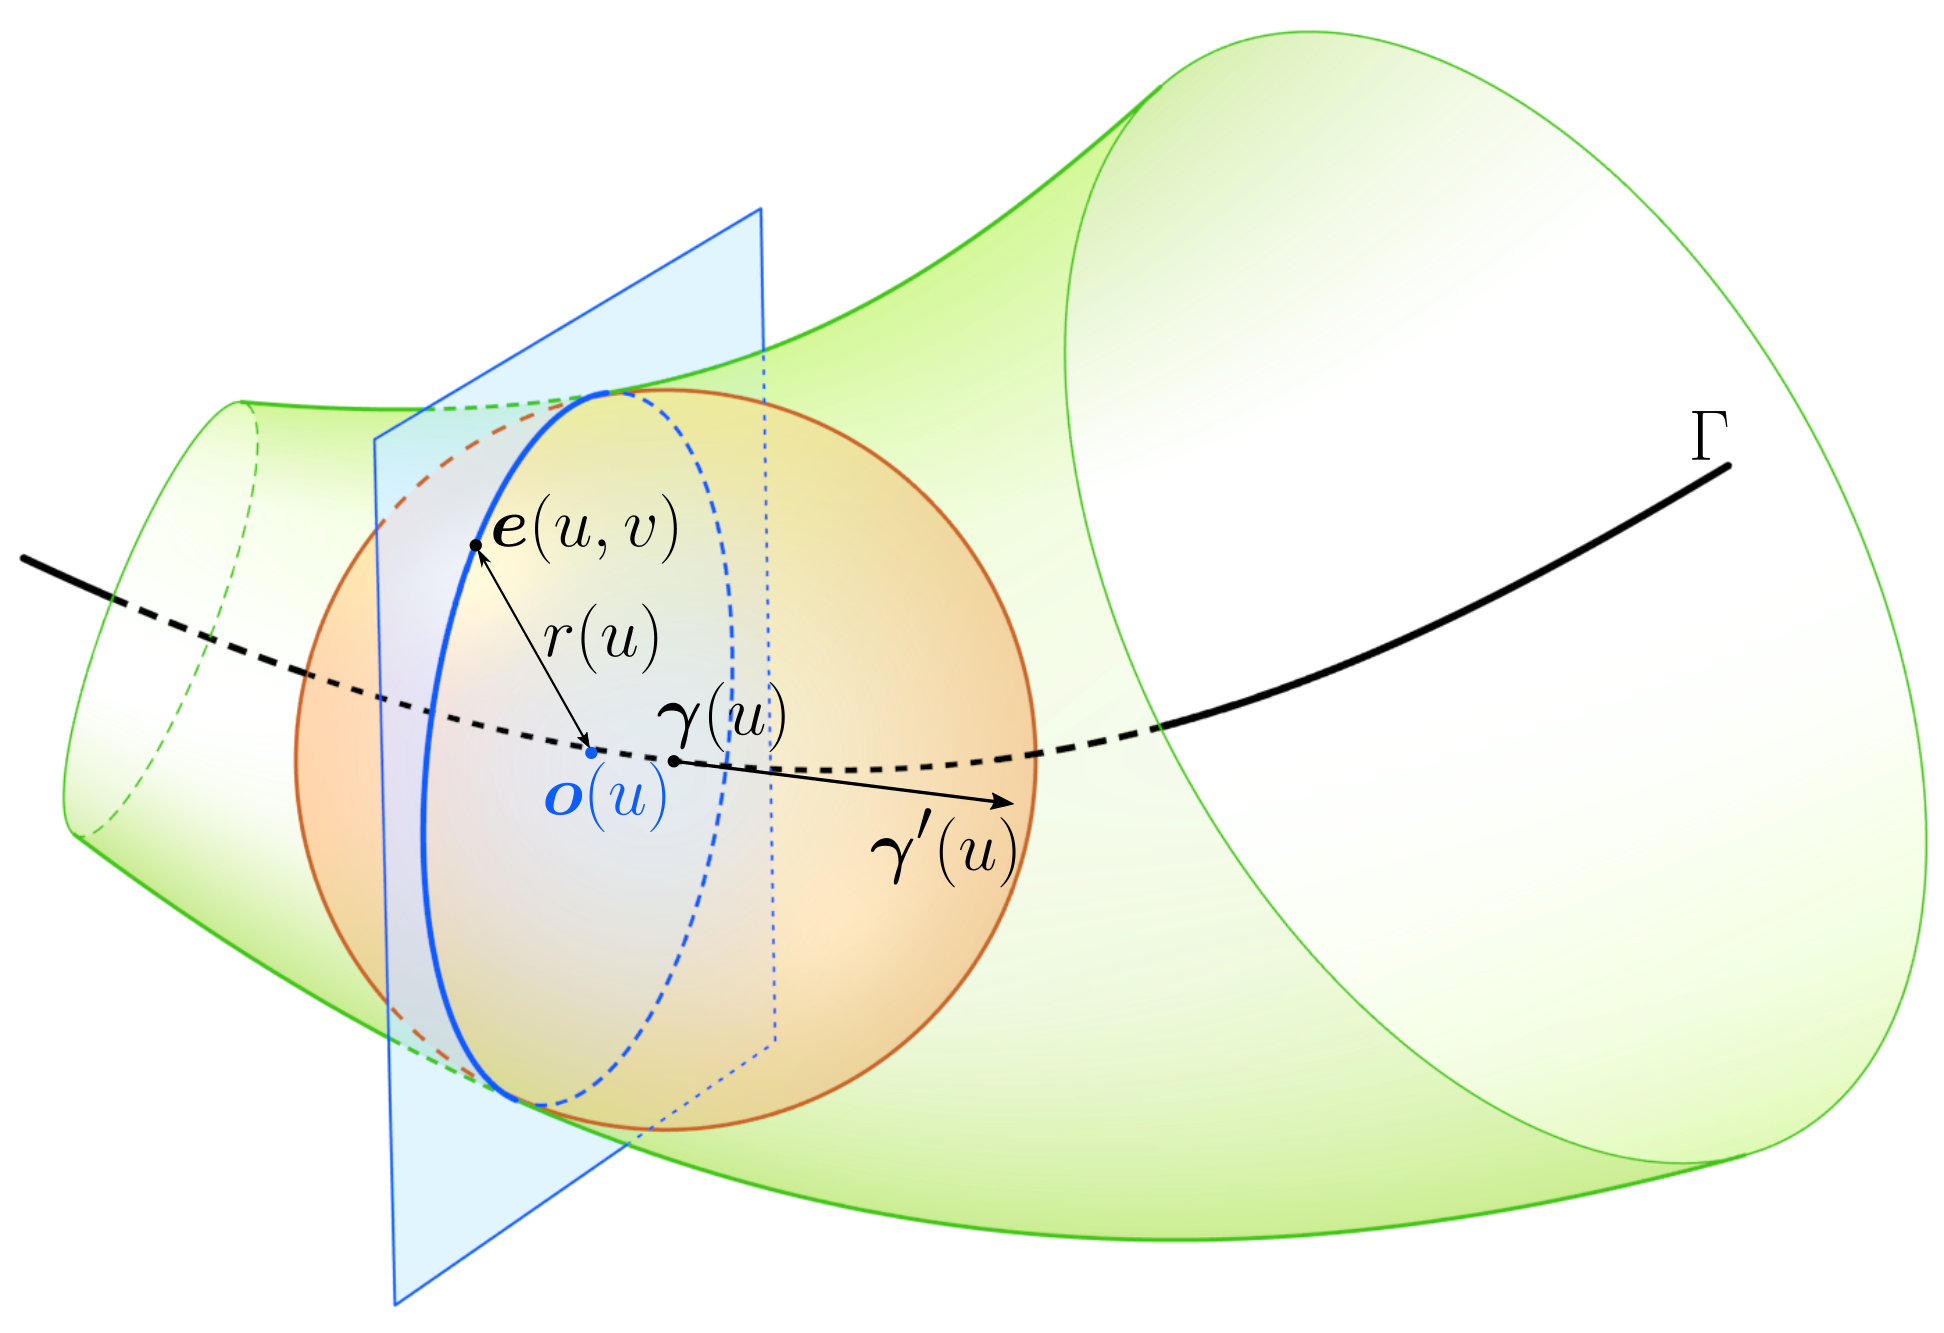
\includegraphics[width=\imagewidth]{figures/images/EdS_propre_courbe.png}};
		\node[coloreos] at (0.55,0.95) {$\EdSpropre{\Gamma}{\rho}$};
		\node[anchor=south west, colorshpere] at (0.46,0.62) {$\sphere[u]$};
	\end{tikzpicture}
	\caption{Paramétrisation de l'EdS propre d'un arc paramétrique.}
\end{figure}
%%Soit $\bg : \wdomain \to \reals^3$ une paramétrisation du support géométrique $\Gamma$ de l'arête $\brepedge$. 
%%L'EdS propre de $\Gamma$ est le lieu des points $\bx \in \reals^3$ qui vérifient
%L'enveloppe $\Phi$ d'une famille de sphères à un paramètre centrées sur une courbe directrice $\Gamma$ est appelée \textit{surface canal} \cite{monge1850}. 
%Si la $\Gamma$ dispose d'une paramétrisation $\bg : \wdomain \to \reals^3$ alors cette surface est le lieu des points $\bx \in \reals^3$ qui vérifient
%\begin{equation}
%  \left\{
%    \begin{matrix}
%        \normtwo{\bx - \bg(u)}^2 - \rho(u)^2 &= 0 ,\\ 
%        \dotprod{\left(  \bx - \bg(u) \right)}{\bg'(u)} + \rho(u)\rho_u(u) &= 0.
%    \end{matrix}
%  \right.
%  \label{eq:sys_canal_surface}
%\end{equation}
Soit $\bg : \wdomain \to \reals^3$ une paramétrisation du support géométrique $\Gamma$ de l'arête $\brepedge$. 
Si l'on considère $\rho$ comme une fonction du paramètre $u$ alors $\EdSpropre{\Gamma}{\rho}$ est le lieu des points $\bx \in \reals^3$ qui vérifient
\begin{equation}
  \left\{
    \begin{matrix}
        \normtwo{\bx - \bg(u)}^2 - \rho(u)^2 &= 0 ,\\ 
        \dotprod{\left(  \bx - \bg(u) \right)}{\bg'(u)} + \rho(u)\rho_u(u) &= 0.
    \end{matrix}
  \right.
  \label{eq:sys_canal_surface}
\end{equation}
A condition que $\rho_u^2 \leq \normtwo{\bg'}^2$, le système \eqref{eq:sys_canal_surface} définit une famille de \textit{cercles caractéristiques}, dont chacun est le lieu des points de tangence entre $\Phi$ et une sphère de la famille $\sphere[\Gamma][\rho]$ (voir figure?).
\par
D'après \eqref{eq:sys_canal_surface}, le cercle caractéristique au point $\bg(u)$ est l'intersection de la sphère $\sphere[u] = \sphere[\bg(u)][\rho(\bg(u))]$ et d'un plan orthogonal à la tangente à $\Gamma$ en ce point (donnée par le vecteur $\bg'(u)$). 
Ce cercle est centré en
\begin{equation}
    \vit{o}(u) = \bg(u) - \frac{\rho(u)\rho_u(u)}{\normtwo{\bg'(u)}^2} \bg'(u),
    \label{eq:cercle_caracteristique_centre}
\end{equation}
et a pour rayon
\begin{equation}
    r(u) = \rho(u) \sqrt{1 - \frac{\rho_u(u)^2}{\normtwo{\bg'(u)}^2}}.
    \label{eq:cercle_caracteristique_rayon}
\end{equation}
\par
Voir $\Phi$ comme une famille cercles caractéristiques permet d'en donner la paramétrisation suivante
\begin{equation}
    \eos(u,v) = \vit{o}(u) + r(u)\vrm{r}(u,v),
    \label{eq:eos_segment_parameterisation}
\end{equation}
où $\vrm{r}$ vérifie
\begin{equation}
	\left\{
		\begin{matrix}
			\normtwo{\vrm{r}} = 1,\\ 
			\dotprod{\vrm{r}}{\bg'} = 0.
		\end{matrix}
	\right.
\end{equation}
De cette façon, les courbes iso-$u$ de $\eos$ sont les cercles caractéristiques.


\subsubsection{Paramétrisation de la pseudo-EdS}
\label{section:parametrisation_pseudo_EdS_arete}
\newcommand{\eosR}{\lo{\vit{\eos}}}
\newcommand{\eosL}{\hi{\vit{\eos}}}

\newcommand{\psiR}{\lo{\vit{\psi}}}
\newcommand{\psiL}{\hi{\vit{\psi}}}







\subsection{Paramétrisation de la pseudo-EdS d'un sommet \brep\ convexe}
2 approches :

\subsubsection{Polygone sphérique découpé en quadrilatères}
\label{section:quadrangulation_polygone_spherique}
avantages/inconvénients :
\begin{itemize}
	\item[$-$] valable seulement si la vitesse normale est uniforme
	\item[$-$] génère plusieurs nouveaux carreaux de surface
	\item[$+$] les nouveaux carreaux sont rectangulaires ($\Rightarrow$ permet l'utilisation de quadratures simples (\cf \autoref{section:clenshaw_curtis_quadrature})
\end{itemize}


\subsubsection{Ajustement de carreau sphérique à un nuage de points}
\label{section:ajustement_carreau_spherique}

\def\s{\vit{s}}

%(\cf notes Huygens)
avantages/inconvénients :
\begin{itemize}
	\item[$-$] le nouveau carreau est restreint
	\item[$+$] valable également si la vitesse normale varie spatialement
	\item[$+$] génère un seul nouveau carreau de surface
\end{itemize}

Soit $\brepvertex$ un sommet \brep\ convexe dont le support géométrique est le point $\p$. 
On cherche à construire un carreau paramétrique restreint décrivant \ie la région de la sphère $\sphere[\p][\rho{\p}]$ délimitée par les arcs de cercles caractéristiques aux extrémités des arêtes \brep\ incidentes à $\p$. 
Afin de simplifier cette construction, on considère que $\p$ est situé à l'origine et que $\rho{\p} = 1$. 
On appliquera la transformation adéquate en fin de construction pour se placer à nouveau dans le cas général. 
\par
Le problème consiste alors, étant donné un ensemble de points $S = \family{\s}{i}{1}{n}$ sur la sphère unité $\mathbb{S}^2$, à construire un carreau paramétrique décrivant une portion $R$ de $\mathbb{S}^2$ contenant $S$. 
On cherche également à minimiser l'aire de $R$ \ldots




\section{Construction d'un modèle \brep\ de l'EdB}

\subsection{Construction du graphe des intersections}
Conservation/création des intersections tangentielles, calcul des intersections transverses entre paire de carreaux non-restreints, segmentation des courbes d'intersection en segments quasi-disjoints (intersection de 3 carreaux non-restreints ou plus), \guillemets{clipping} par le domaine paramétrique de chaque carreau restreint
\par\bigskip
pour un carreau de surface, il s'agit d'un graphe planaire orienté dont un plongement dans $\reals^2$ est donné par la trace des courbes d'intersections dans son espace paramétrique

\begin{figure}
\centering
\plotCurvedDirectedGraph{/d/bandrieu/GitHub/FFTsurf/test/graph/graph_bezier_control_points.dat}{25mm}
\caption{Plongement du graphe des intersections dans l'espace paramétrique d'un carreau de surface.}
\end{figure}


\subsection{Construction des faces, arêtes et sommets \brep}
pour chaque carreau : extraction des cycles du graphe d'intersection, caractérisations des contours (extérieurs/intérieurs), détermination des faces $\to$ insertion des contours dans la \brep\ $\to$ insertion des (co-)arêtes et sommets
\begin{figure}
	\centering
	\newcommand{\arc}{\mathcal{A}}%
\newcommand{\subin}{\ensuremath{_{\mathrm{in}}}}%
\newcommand{\subout}{\ensuremath{_{\mathrm{out}}}}%
\newcommand{\noeud}{\mathcal{N}}%
\newcommand{\cycle}{\mathcal{C}}%
\newcommand{\graph}{\mathcal{G}}%
\begin{tikzpicture}[%
	scale=0.5,
	>={Latex[length=4pt]},      % Arrow style
    start chain=going below,    % General flow is top-to-bottom
    node distance=6mm and 50mm, % Global setup of box spacing
    every join/.style={flow},   % Default linetype for connecting boxes
    ]
% ------------------------------------------------- 
% A few box styles 
% <on chain> *and* <on grid> reduce the need for manual relative
% positioning of nodes
\tikzset{
  base/.style={draw, on chain, on grid, align=center, minimum height=4ex, minimum width=5em},
  proc/.style={base, rectangle},
  test/.style={base, diamond, aspect=2},
  term/.style={proc, rounded corners=2ex},
  % coord node style is used for placing corners of connecting lines
  coord/.style={coordinate, on chain, on grid, node distance=6mm and 25mm},
  % -------------------------------------------------
  % Connector line styles for different parts of the diagram
  flow/.style={->, draw}
}
% -------------------------------------------------
\node [term, join] (start) {Début};
\node [proc, join] (p1) {Éliminer les branches pendantes de $\graph$};
\node [test, join] (t1) {$A = \emptyset$ ?};

\node [proc] (startarc) {Choisir un arc $\arc_*$ de $\graph$};

\node [proc, join] {Démarrer un nouveau cycle $\cycle$ à partir de $\arc_*$};
\node [proc, join] {$\arc \leftarrow \arc_*$ et\\ $\noeud \leftarrow \dest(\arc)$};


\node [test, join] (t2) {$\noeud = \orig(\arc_*)$?};

\node [proc] (maxangles) {Identifier $\hi{\alpha}\subin$, $\hi{\alpha}\subout$ et $\hi{\arc}\subout$};


\node [test, join] (t3) {$\hi{\alpha}\subin > \hi{\alpha}\subout$ ?};
\node [proc] (abortcycle) {Abandonner $\cycle$};

\node [term, left=of t1, text width=3em] (end) {Fin};
\node [proc, right=of t2] (completecycle) {Rajouter $\cycle$\\à la liste des cycles\\et l'extraire de $\graph$};
\node [proc, left=of t3] (appendcycle) {$\arc \leftarrow \hi{\arc}\subout$,\\ $\noeud \leftarrow \dest(\arc)$ et \\ajouter $\arc$ à $\cycle$};


\draw [flow] (t1.west) -- node[above] {oui} (end);
\draw [flow] (t1.south) -- node[left] {non} (startarc);

\draw [flow] (t2.east) -- node[above] {oui} (completecycle);
\draw [flow] (t2.south) -- node[left] {non} (maxangles);

\draw [flow] (t3.west) -- node[above] {oui} (appendcycle);
\draw [flow] (t3.south) -- node[left] {non} (abortcycle);


\draw [flow] (appendcycle.north) |- (t2);

\node [coord, left=of appendcycle] (c2)  {};
\draw [flow] (abortcycle.west) -| (c2) |- (p1);

\draw [flow] (completecycle.north) |- (p1);
% -------------------------------------------------
\end{tikzpicture}
	\caption{Organigramme de l'algorithme d'extraction des cycles d'un graphe orienté plongé dans $\reals^2$.}
\end{figure}


\begin{figure}
	\centering
	\setlength{\imagewidth}{60mm}%
\setlength{\imageheight}{\imagewidth}%
%
\colorlet{facecolor1}{mycolor_1}
\colorlet{facecolor2}{mycolor_2}
\colorlet{facecolor3}{mycolor_3}
%
\begin{tikzpicture}[
	x=0.5\imagewidth, 
	y=0.5\imageheight,
	halfedge/.style={
		line width=0.8pt, 
		line cap=round, 
		-{Triangle[left]}
	},
]
	%\input{/d/bandrieu/GitHub/FFTsurf/test/graph/graph_faces_tikzcode.tex}
	\input{../../FFTsurf/test/graph/graph_faces_tikzcode.tex}
\end{tikzpicture}

	\caption{Faces du graphe}
\end{figure}